%----------------------------------------------------------------------------
\section{Model-based Systems Engineering}\label{sec:mbse}
%----------------------------------------------------------------------------

The INCOSE SE Vision 2020\cite{incose-systems-engineering-2020} defines Model-based systems engineering (MBSE) as:

\blockquote{the formalized application of modeling to support system requirements, design, analysis, verification and validation activities beginning in the conceptual design phase and continuing throughout development and later life cycle phases. MBSE is part of a long-term trend toward model-centric approaches adopted by other engineering disciplines, including mechanical, electrical and software. In particular, MBSE is expected to replace the document-centric approach that has been practiced by systems engineers in the past and to influence the future practice of systems engineering by being fully integrated into the definition of systems engineering processes.}

Applying MBSE is expected to provide significant benefits over the document centric approach by enhancing productivity and quality, reducing risk, and providing improved communications among the system development team.\cite{omgwiki}

In MBSE, one of the most important concepts is the term "model" itself. In the literature it has many different definitions:

\begin{enumerate}
	\item A physical, mathematical, or otherwise logical representation of a system, entity, phenomenon, or process.\cite{DoD_modeling_and_simulation}\label{item:dod}
	\item A representation of one or more concepts that may be realized in the physical world.\cite{sysml_practical_guide}
	\item A simplified representation of a system at some particular point in time or space intended to promote understanding of the real system.\cite{modsim}
	\item An abstraction of a system, aimed at understanding, communicating, explaining, or designing aspects of interest of that system.\cite{object-process-methodology}
	\item A selective representation of some system whose form and content are chosen based on a specific set of concerns. The model is related to the system by an explicit or implicit mapping.\cite{ORMSC/2010-09-06}
\end{enumerate}

As one can see, choosing a definition is very much dependent upon how we wish to use our "model"; in this work I will use the number \ref{item:dod} definition.

\subsection{Systems Modeling Language}\label{ssec:sysml}

Systems Modeling Language (OMG SysML)\cite{omg_sysml} is a general-purpose modeling language that supports the specification, design, analysis, and verification of systems that may include harware and equipment, software, data, personnel, procedures, and facilities. SysML is a graphical modeling language with a semantic foundation for representing requirements, behaviour, structure, and properties of the system and its components.\cite{sysml_practical_guide}

This work focuses only on the \emph{behavioural} modeling tools SysML provides. In the following section, I present two of the most used concepts.

\subsubsection{State Machine}

Reactive systems are all around us in our daily lives; in smart phones, avionics systems or event our calculators. Frequently, reactive systems appear in areas, where safety-critical operation is crucial, as even the slightest
misbehaviour can have catastrophic consequences. This makes the verification of these systems a must during their design process.

The defining characteristic of reactive systems is their event-driven nature, which means that they continuously receive external stimuli (events), based on which they change their internal state and possibly react with some output\cite{10.1007/978-3-642-82453-1_17}. Reactive systems can be verified using model checking techniques (see \autoref{sec:formal_verification}). Statecharts\cite{HAREL1987231} are a popular and intuitive language to capture the behaviour of reactive systems \cite{10.1145/3417990.3421407, 10.1007/978-3-319-11653-2_10}, and are at the same time formal and rigorous. 

\begin{figure}[!ht]
	\centering
	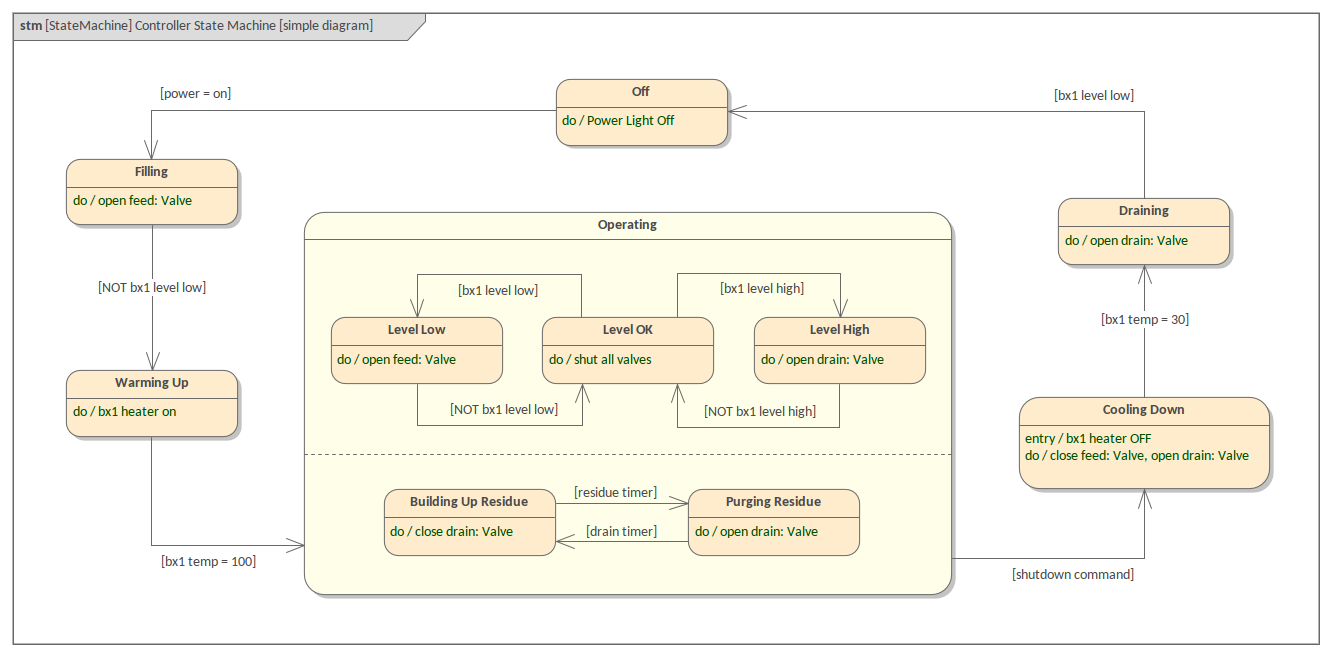
\includegraphics[width=67mm, keepaspectratio]{figures/sysml_state_machine.png}\hspace{1cm}
	\caption{A SysML State Machine.}
	\label{fig:sysml_state_machine}
\end{figure}

SysML state machines (see \ref{fig:sysml_state_machine}) extend the concept of statecharts with hierarchical state-refinement, orthogonal regions, action-effect behaviour and state machine composition (explained in more detail in \autoref{ssec:composite-systems}). These advanced constructs make state machines easy to use for engineers, but lead to the formal verification process being challenging. This challenge can be overcome using a transformation tool, such as Gamma, of which I will be talking in \autoref{sec:gamma}.

\subsubsection{Activity Diagram}\label{ssec:sysml_activity}

Reactive systems however cannot describe the complicated semantics of distributed systems with concurrent, parallel behaviour, where the \emph{interesting} thing is what the system \emph{does} step-by-step. SysML activity diagrams are a primary representation for modeling process based behaviour\cite{omg_sysml} for distributed, concurrent systems. \autoref{fig:sysml_activity_artifacts} shows the set of interesting artifacts used in this work. In the following, I will introduce the different artifacts and show an example of a SysML activity diagram.

\begin{figure}[!ht]
	\centering
	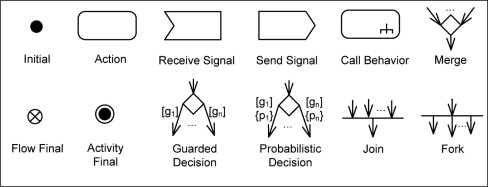
\includegraphics[width=100mm, keepaspectratio]{figures/sysml_activity_artifacts.png}\hspace{1cm}
	\caption{Artifacts of SysML activity diagrams.}
	\label{fig:sysml_activity_artifacts}
\end{figure}

SysML activity diagram is a graph based diagram, where the nodes are connected via flows. The dynamic behaviour of activity diagrams comes from \emph{tokens} travelling from node to node; based on the given node's semantics a connected flow removes tokens from the source node and puts them onto the target node.

A \emph{control} token is a simple token without any value associated with it, a \emph{data} token is a token that contains some value. 
The difference between the nodes capture the various behaviours a given activity diagram can model.
Simple \textbf{actions} represents a single step of behaviour that converts a set of inputs to a set of outputs Both inputs and outputs are specified as pins. Behaviour is represented as a flow of tokens, the flow is started from the initial node, which generates and passes a token to each node to which it is connected. Fork nodes generate tokens on all of its leaving paths, and join nodes generate a token on the leaving path when all entering paths have at least one token. Merge nodes consume all incoming tokens, and only sends out one on its outgoing flows, likewise, decision nodes take one token from its input flows, and sends it out on its one and only one enabled outflows.
There are two kinds of flows, control and object flows. Control tokens travel through control flows, and data tokens travel through object flows. Object flows must start from an output pin, and must end with an input pin. The execution of an activity diagram ends when the activity final node receives a token. The detailed specification can be found in OMG\cite{omg_sysml}.

\textit{Activity example description, and figure. This example will be used for all activity examples.}

\iffalse
\subsubsection{Differences and Combination}

State Machines are a popular [1, 2] language to capture the behaviour
of reactive systems\cite{HAREL1987231} that react to external stimuli depending on
their internal state. Stat Machines provide an expressive formalism to
represent complex \emph{state-based} behaviour by introducing hierarchical
state refinement, memory (variables and history state) and complex
transitions (e.g., fork and join transitions).

As contrast, Activities model the behaviour of distributed systems with many interconnecting components, all running in parallel; said components may have dependencies on each other (one calculates a value the other needs), or have a limited resources (a factory only has one worker).

SysML provides a functionality to combine different behaviours, using the \emph{call behaviour} pattern. By using a call behaviour action inside a State Machine, we are able to combine the behaviour of the two. This is the basis of composite behaviour models, and the motivation of this work. 
\fi